% CS615A Aspects of System Administration
% Author: Jan Schaumann <jschauma@netmeister.org>
% $Id: slides.tex,v 1.12 2006/02/12 23:15:03 jschauma Exp $

\special{! TeXDict begin /landplus90{true}store end }

\documentclass[xga]{xdvislides}
\usepackage[landscape]{geometry}
\usepackage{graphics}
\usepackage{graphicx}
\usepackage{colordvi}
\usepackage{tabularx}
\usepackage{multirow}

\newcommand{\gargantuan}{\fontsize{100}{105}\selectfont}

\begin{document}
\setfontphv

%%% Headers and footers
\lhead{\slidetitle}                               % default:\lhead{\slidetitle}
\chead{CS615 - Aspects of System Administration}% default:\chead{\relax}
\rhead{Slide \thepage}                       % default:\rhead{\sectiontitle}
\lfoot{\Gray{Documentation, Multiuser Basics}}% default:\lfoot{\slideauthor}
\cfoot{\relax}                               % default:\cfoot{\relax}
\rfoot{\Gray{\today}}

\vspace*{\fill}
\begin{center}
	\Hugesize
		CS615 - Aspects of System Administration\\ [1em]
		Documentation, Multiuser Basics\\ [1em]
	\hspace*{5mm}\blueline\\ [1em]
	\Normalsize
		Department of Computer Science\\
		Stevens Institute of Technology\\
		Jan Schaumann\\
		\verb+jschauma@stevens.edu+\\
		\verb+http://www.cs.stevens.edu/~jschauma/615/+
\end{center}
\vspace*{\fill}

\subsection{Homework}
Review your submissions.  Ask yourself:
\begin{itemize}
	\item What's the difference in output across operating systems?
	\item What do the different numbers mean?
	\item Why did I open access to port 80?
	\item Why does Solaris mount libc?
	\item Why does {\tt fdisk(8)} claim that {\tt /dev/xvde1 doesn't
		contain a valid partition table}?
	\item Why does Solaris say things like {\tt /dev/dsk/c3d0s0 is
		part of active ZFS pool rpool. Please see zpool(1M).} ?
	\item Why do Solaris partitions show as {\tt unassigned}?
	\item Which partitions are overlapping?  Why?
	\item Do the numbers I produced match?  Do they make sense?
\end{itemize}

\subsection{Homework}
Review your submissions.  Ask yourself:
\vfill
\Huge
\begin{center}
       When I look for information, do I pay attention or do I just copy
       whatever is written on some website?
\end{center}
\Normalsize
\vfill

\subsection{Documentation Techniques}
\vfill
\begin{center}
\Huge
Yes, you should write documentation. \\
\small
(Emphasis on either word optional.)
\Normalsize
\end{center}
\vfill

\subsection{Documentation Techniques}
Why?
\begin{itemize}
	\item ``this is: ...''
	\item ``this is why...''
	\item ``this is how...''
	\item ``just so you know...''
	\item ``in case you're interested...''
\end{itemize}

\subsection{Documentation Techniques}
Why?
\begin{itemize}
	\item so you don't forget
	\item so users know how to use the system
	\item so other administrators can repeat what you've done
	\item so {\em you} can repeat what you've done
	\item so you actually do things right
\end{itemize}

\subsection{Documentation Techniques}
Types of documents:

\begin{itemize}
	\item HOWTO
	\item policies
	\item architecture / design
	\item program documentation / specification
	\item runbook
	\item research
\end{itemize}


\subsection{Documentation Techniques}
Basics:
\begin{itemize}
	\item know your target audience
	\item don't make assumptions
	\item explicitly note your assumptions
	\item include pointers/references to your assumptions
	\item include screen captures where appropriate
	\item include verbatim examples to illustrate common use
\end{itemize}

\subsection{Documentation Techniques}
Documentation is an {\em ongoing} task.

\begin{itemize}
	\item keep track of changes (use a revision control system)
	\item date your documents
\end{itemize}

\vspace{.25in}
Documentation is a {\em collaborative} task.

\begin{itemize}
	\item ensure remote access
	\item ensure distributed collaboration
	\item ensure platform/version independence
\end{itemize}

\vspace{.25in}
Documentation is an {\em accumulative} task.

\begin{itemize}
	\item make sure you have a searchable index
	\item identify and flag out-dated documentation
	\item remove false or unhelpful documentation
\end{itemize}

\newpage
\vspace*{\fill}
\begin{center}
    \Hugesize
        Of Users and Groups\\ [1em]
    \hspace*{5mm}
    \blueline\\
    \hspace*{5mm}\\
	...and Trust
\end{center}
\vspace*{\fill}

\subsection{You are a Super User!}
\begin{center}
	
\includegraphics[scale=1.0]{pics/superman.eps} \\
	\small
	Yes, you are!
	\Normalsize
\end{center}

\subsection{You are a Super User!}
\begin{center}
	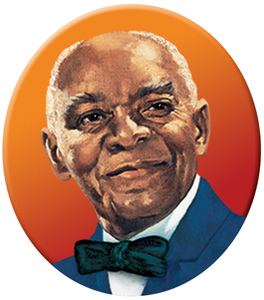
\includegraphics[scale=4.0]{pics/uncle-ben.eps} \\
	\addvspace{.2in}
	\Huge
	``With great power comes great responsibility.''
	\Normalsize
\end{center}

\subsection{Implications of a Multi-User System}
\vspace*{\fill}
\begin{center}
	\includegraphics[scale=0.8]{pics/teamwork.eps}
\end{center}
\vspace*{\fill}

\subsection{Implications of a Multi-User System}
\vspace*{\fill}
\begin{center}
	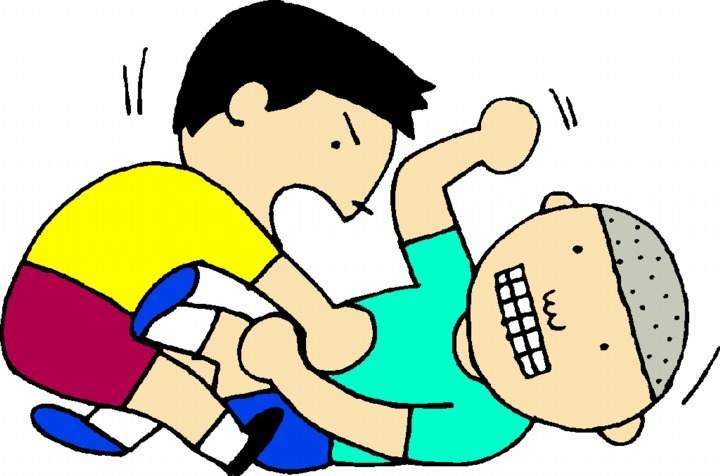
\includegraphics[scale=0.7]{pics/kids_fighting.eps}
\end{center}
\vspace*{\fill}

\subsection{Consider Scalability}
Things to consider:
\\

\begin{center}
	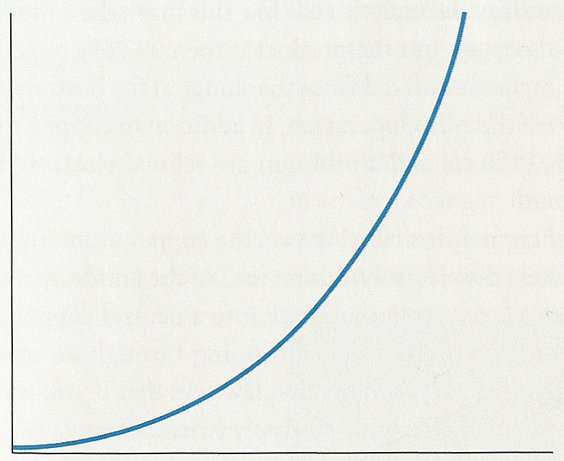
\includegraphics[scale=2.8]{pics/exponential_growth.eps}
\end{center}


\subsection{Granting Privileges requires Trust}
\begin{itemize}
	\item different environments have different trust models
	\item human interactions in small groups strengthen trust
	\item larger groups are divided into smaller, close-nit groups
	\item the more groups you have, the weaker their trust bonds are
\end{itemize}

\subsection{Granting Privileges requires Trust}
\begin{itemize}
	\item different environments have different trust models
	\item human interactions in small groups strengthen trust
	\item larger groups are divided into smaller, close-nit groups
	\item the more groups you have, the weaker their trust bonds are
\end{itemize}
\vspace{.5in}

\begin{center}
	\Huge
	{\bf Trust does not scale.}
	\Normalsize
\end{center}

\subsection{Granting Privileges requires Trust}
\vfill
\begin{center}
	\Huge
	Trust, but (be able to) verify.
	\Normalsize
\end{center}
\vfill



\subsection{Implications of a Multi-User System}
\vspace*{\fill}
\begin{center}
	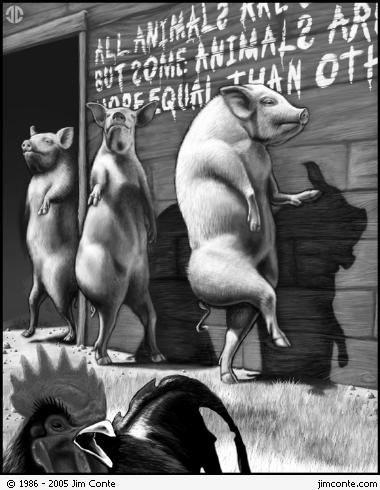
\includegraphics[scale=0.9]{pics/animal_farm.eps}
\end{center}
\vspace*{\fill}

\subsection{Implications of a Multi-User System}
\begin{itemize}
	\item users may want to keep files private
\end{itemize}

\subsection{Implications of a Multi-User System}
\begin{itemize}
	\item users may want to keep files private
	\item users may want to share files
\end{itemize}

\subsection{Implications of a Multi-User System}
\begin{itemize}
	\item users may want to keep files private
	\item users may want to share files
	\item users may (try to gain) access to files they shouldn't have access to
\end{itemize}

\subsection{Implications of a Multi-User System}
\begin{itemize}
	\item users may want to keep files private
	\item users may want to share files
	\item users may (try to gain) access to files they shouldn't have access to
	\item users may (want to) do things that affect other users
\end{itemize}

\subsection{Implications of a Multi-User System}
\begin{itemize}
	\item users may want to keep files private
	\item users may want to share files
	\item users may (try to gain) access to files they shouldn't have access to
	\item users may (want to) do things that affect other users
	\item different users may require different privileges
\end{itemize}

\subsection{Users and User-IDs}
\begin{center}
	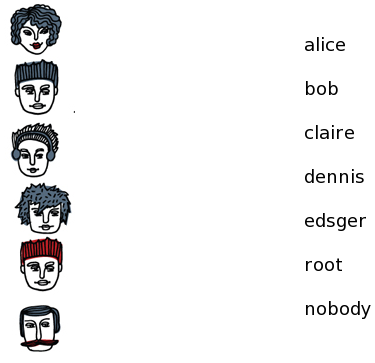
\includegraphics[scale=0.9]{pics/user-sets0.eps} \\
	One-to-one?  Onto?
\end{center}

\subsection{Users and User-IDs}
\begin{center}
	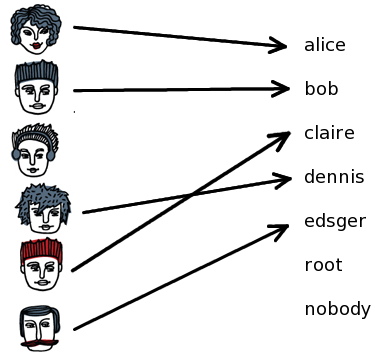
\includegraphics[scale=0.9]{pics/user-sets1.eps} \\
	{\em Not} onto!
\end{center}

\subsection{Users and User-IDs}
\begin{center}
	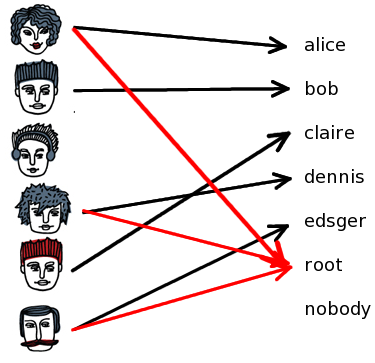
\includegraphics[scale=0.9]{pics/user-sets2.eps} \\
	{\em Not} one-to-one, either!
\end{center}

\subsection{Users and User-IDs}

\begin{center}
	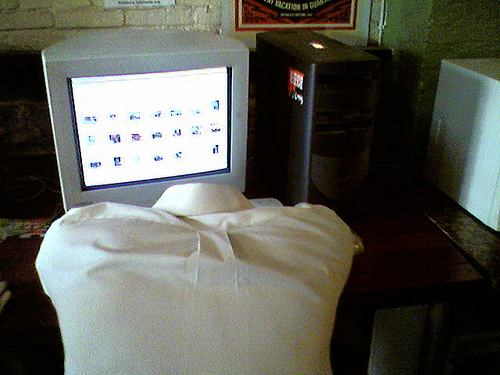
\includegraphics[scale=0.8]{pics/headless.eps} \\
	{\tt nobody}
\end{center}

\subsection{UNIX Fundamentals: User Accounts and File Permissions}
Every account
\begin{itemize}
	\item has a {\em unique} ID
	\item belongs to at least one group
	\item may or may not be password protected
	\item may or may not have a valid login program
\end{itemize}

\subsection{UNIX Fundamentals: User Accounts and File Permissions}
Every account
\begin{itemize}
	\item has a {\em unique} ID
	\item belongs to at least one group
	\item may or may not be password protected
	\item may or may not have a valid login program
\end{itemize}
\addvspace{.5in}
Every file
\begin{itemize}
	\item is associated with a {\em uid} and a {\em gid}
	\item has a number of protection bits
\end{itemize}

\subsection{UNIX Fundamentals: User Accounts and File Permissions}
\vfill
\begin{center}
	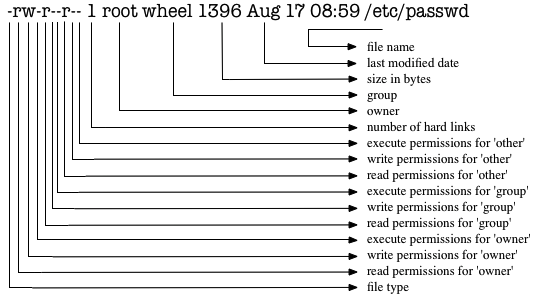
\includegraphics[scale=0.9]{pics/ls-l.eps}
\end{center}
\vfill



\subsection{Unix Groups}
\begin{itemize}
	\item enables {\em arbitrary} collections of users to share resources
	\item information stored in \verb+/etc/group+, format is: \\
		\verb+name:*:GID:user1,user2,...+
	\item most Unix systems impose a limit of 16 or 32 group memberships per
		user
	\item most Unix systems have a common default group for new users (some
		Linux versions deviate)
	\item some Unix systems have group shadow files
\end{itemize}

\subsection{Group Access}
At any but the smallest environments, we find:
\begin{itemize}
	\item a central user database
	\item users divided into different access groups
	\item access to systems is granted primarily by such group membership
	\item privileges on a system are also granted by such group membership
\end{itemize}

\subsection{Group Access}
\begin{center}
	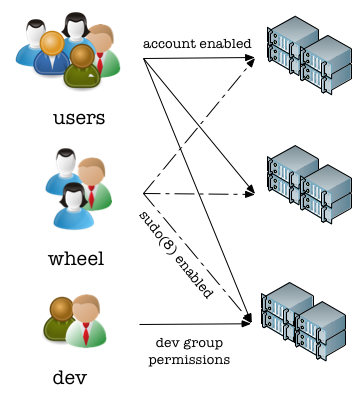
\includegraphics[scale=0.8]{pics/groups-machines.eps}
\end{center}


\subsection{Adding and Removing Accounts}
\begin{center}
	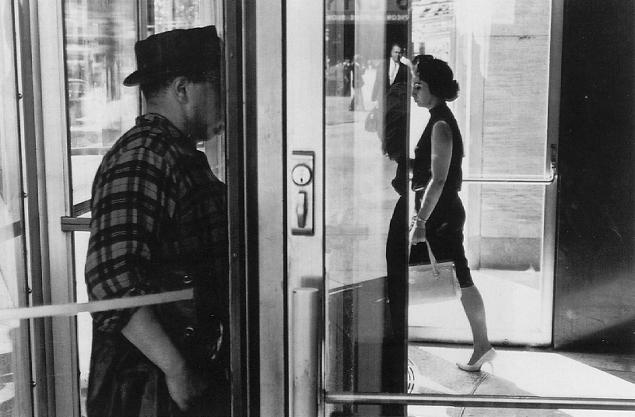
\includegraphics[scale=0.8]{pics/friedlander_revolving_door.eps}
\end{center}

\subsection{Adding and Removing Accounts}
\vfill
Accounts management is done centrally; changes are applied to machines via a
configuration management system and/or directory service.
\vfill

\subsection{Adding accounts}
Things to consider:
\begin{itemize}
	\item create/assign username, UID, primary group, supplementary groups,
		choose shell
\end{itemize}

\subsection{Adding accounts}
Things to consider:
\begin{itemize}
	\item create/assign username, UID, primary group, supplementary groups,
		choose shell
	\item assign a password
\end{itemize}

\subsection{Adding accounts}
Things to consider:
\begin{itemize}
	\item create/assign username, UID, primary group, supplementary groups,
		choose shell
	\item assign a password
	\item create a home directory
\end{itemize}

\subsection{Adding accounts}
Things to consider:
\begin{itemize}
	\item create/assign username, UID, primary group, supplementary groups,
		choose shell
	\item assign a password
	\item create a home directory
	\item place initialialization files in the user's home directory
\end{itemize}

\subsection{Adding accounts}
Things to consider:
\begin{itemize}
	\item create/assign username, UID, primary group, supplementary groups,
		choose shell
	\item assign a password
	\item create a home directory
	\item place initialialization files in the user's home directory
	\item set other parameters (password aging, resource limits...)
\end{itemize}

\subsection{Adding accounts}
Things to consider:
\begin{itemize}
	\item create/assign username, UID, primary group, supplementary groups,
		choose shell
	\item assign a password
	\item create a home directory
	\item place initialialization files in the user's home directory
	\item set other parameters (password aging, resource limits...)
	\item add user to other facilities (enable disk quota, mail filters,
		printer subsystem...)
\end{itemize}

\subsection{Adding accounts}
Things to consider:
\begin{itemize}
	\item create/assign username, UID, primary group, supplementary groups,
		choose shell
	\item assign a password
	\item create a home directory
	\item place initialialization files in the user's home directory
	\item set other parameters (password aging, resource limits...)
	\item add user to other facilities (enable disk quota, mail filters,
		printer subsystem...)
	\item perform any other site-specific initialization tasks
\end{itemize}

\subsection{Disabling and Removing User Accounts}
Things to consider:
\begin{itemize}
	\item change other passwords
\end{itemize}

\subsection{Disabling and Removing User Accounts}
Things to consider:
\begin{itemize}
	\item change other passwords
	\item terminate running processes
\end{itemize}

\subsection{Disabling and Removing User Accounts}
Things to consider:
\begin{itemize}
	\item change other passwords
	\item terminate running processes
	\item remove user from secondary groups
\end{itemize}

\subsection{Disabling and Removing User Accounts}
Things to consider:
\begin{itemize}
	\item change other passwords
	\item terminate running processes
	\item remove user from secondary groups
	\item (re)define a mail alias or redirect mail
\end{itemize}

\subsection{Disabling and Removing User Accounts}
Things to consider:
\begin{itemize}
	\item change other passwords
	\item terminate running processes
	\item remove user from secondary groups
	\item (re)define a mail alias or redirect mail
	\item remove any cronjobs or other pending tasks for that user
\end{itemize}

\subsection{Disabling and Removing User Accounts}
Things to consider:
\begin{itemize}
	\item change other passwords
	\item terminate running processes
	\item remove user from secondary groups
	\item (re)define a mail alias or redirect mail
	\item remove any cronjobs or other pending tasks for that user
	\item backup all of the users files
\end{itemize}

\subsection{Disabling and Removing User Accounts}
Things to consider:
\begin{itemize}
	\item change other passwords
	\item terminate running processes
	\item remove user from secondary groups
	\item (re)define a mail alias or redirect mail
	\item remove any cronjobs or other pending tasks for that user
	\item backup all of the users files
	\item perform any other site-specific tasks
\end{itemize}

\subsection{Practical Policies}

\begin{center}
	
\includegraphics[scale=0.7]{pics/documents.eps}
\end{center}

\subsection{Practical Policies}
Some important policy documents you may need:
\begin{itemize}
	\item service level agreements (SLAs) for routine tasks
	\item administrative service policies
	\item rights and responsibilities of users
	\item policies regarding sysadmin or other users with special
		privileges
	\item guest account policies
	\item disaster recovery plan
	\item security incidence response plan
	\item software licensing (inbound, in-house, outbound)
	\item ...
\end{itemize}

\subsection{Practical Policies}
\begin{center}
	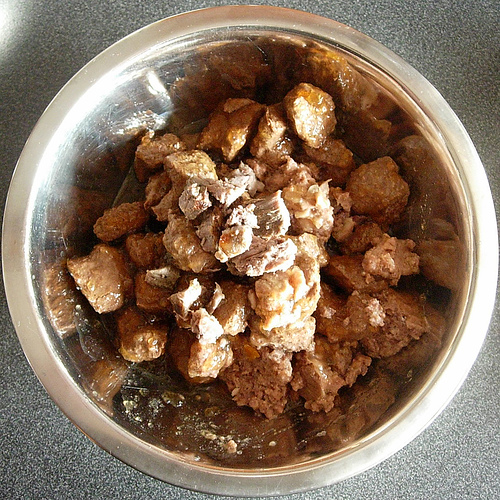
\includegraphics[scale=0.9]{pics/dogfood.eps}
\end{center}

\subsection{Policy Enforcement}
In order to enforce a policy you need to make sure, that
\begin{itemize}
	\item all involved parties are informed of the policy
\end{itemize}

\subsection{Policy Enforcement}
In order to enforce a policy you need to make sure, that
\begin{itemize}
	\item all involved parties are informed of the policy
	\item you log relevant information
\end{itemize}

\subsection{Policy Enforcement}
In order to enforce a policy you need to make sure, that
\begin{itemize}
	\item all involved parties are informed of the policy
	\item you log relevant information
	\item logs cannot be tempered with and are secure
\end{itemize}

\subsection{Policy Enforcement}
In order to enforce a policy you need to make sure, that
\begin{itemize}
	\item all involved parties are informed of the policy
	\item you log relevant information
	\item logs cannot be tempered with and are secure
	\item you have buy-in from all stakeholders
\end{itemize}

\subsection{Ethics}
\begin{center}
	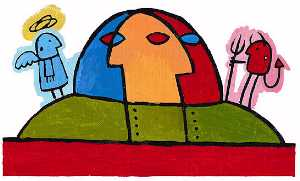
\includegraphics[scale=2.5]{pics/angel-devil.eps}
\end{center}

\subsection{Ethics}
The LISA Code of Ethics:
\\

\newcolumntype{S}{>{\centering\arraybackslash} m{.4\linewidth} }
\begin{tabular}{ p{10cm} S }
\begin{itemize}
	\item Professionalism
	\item Personal Integrity
	\item Privacy
	\item Laws and Policies
	\item System Integrity
	\item Education
	\item Social Responsibility
	\item Ethical Responsibility
\end{itemize}
& \multirow{20}{*}{
\includegraphics[scale=1.3]{pics/angel.eps}} \\
\end{tabular}

\subsection{Ethics: Professionalism}
\vfill
\begin{center}
I will maintain professional conduct in the workplace and will not allow
personal feelings or beliefs to cause me to treat people unfairly or
unprofessionally.
\end{center}
\vfill

\subsection{Ethics: Personal Integrity}
\vfill
\begin{center}
I will be honest in my professional dealings and forthcoming about my
competence and the impact of my mistakes. I will seek assistance from
others when required. \\
\vspace{.5in}

I will avoid conflicts of interest and biases whenever possible. When my
advice is sought, if I have a conflict of interest or bias, I will declare
it if appropriate, and recuse myself if necessary.
\end{center}
\vfill


\subsection{Ethics: Privacy}
\vfill
\begin{center}
I will access private information on computer systems only when it is
necessary in the course of my technical duties. I will maintain and
protect the confidentiality of any information to which I may have access,
regardless of the method by which I came into knowledge of it.
\end{center}
\vfill

\subsection{Ethics: Laws and Policies}
\vfill
\begin{center}
I will educate myself and others on relevant laws, regulations, and
policies regarding the performance of my duties.
\end{center}
\vfill

\subsection{Ethics: Communication}
\vfill
\begin{center}
I will communicate with management, users, and colleagues about computer
matters of mutual interest. I will strive to listen to and understand the
needs of all parties.
\end{center}
\vfill

\subsection{Ethics: System Integrity}
\vfill
\begin{center}
I will strive to ensure the necessary integrity, reliability, and
availability of the systems for which I am responsible. \\
\vspace{.5in}

I will design and maintain each system in a manner to support the
purpose of the system to the organization.
\end{center}
\vfill

\subsection{Ethics: Education}
\vfill
\begin{center}
I will continue to update and enhance my technical knowledge and other
work-related skills. I will share my knowledge and experience with others.
\end{center}
\vfill

\subsection{Ethics: Responsibility to the Computing Community}
\vfill
\begin{center}
I will cooperate with the larger computing community to maintain the
integrity of network and computing resources.
\end{center}
\vfill

\subsection{Ethics: Social Responsibility}
\vfill
\begin{center}
As an informed professional, I will encourage the writing and adoption of
relevant policies and laws consistent with these ethical principles.
\end{center}
\vfill

\subsection{Ethics: Ethical Responsibility}
\vfill
\begin{center}
I will strive to build and maintain a safe, healthy, and productive
workplace. \\
\vspace{.5in}

I will do my best to make decisions consistent with the safety, privacy,
and well-being of my community and the public, and to disclose promptly
factors that might pose unexamined risks or dangers. \\
\vspace{.5in}

I will accept and offer honest criticism of technical work as appropriate
and will credit properly the contributions of others. \\
\vspace{.5in}

I will lead by example, maintaining a high ethical standard and degree
of professionalism in the performance of all my duties. I will support
colleagues and co-workers in following this code of ethics.

\end{center}
\vfill

\subsection{At the end of the day...}
\begin{center}
	
\includegraphics[scale=0.5]{pics/thumbsup-borat.eps}
\end{center}

\subsection{Reading}
User Management:
\begin{itemize}
	\item {\em Frisch}: Ch 6; {\em Burgess}: Ch 5;
	\item \verb+passwd(5)+, \verb+passwd.conf(5)+, \verb+login.conf(5)+,
		\verb+vipw(8)+
	\item \verb+group(5)+
	\item \verb+useradd(8)+, \verb+usermod(8)+, \verb+user(8)+,
		\verb+usermgmt.conf(5)+
	\item \verb+userdel(8)+
\end{itemize}
\vspace{.5in}
\begin{itemize}
	\item http://www.dartmouth.edu/~rc/help/faq/permissions.html
	\item http://nixsrv.com/llthw/ex23
\end{itemize}

\subsection{Reading}
Ethics:
\begin{itemize}
	\item \verb+https://www.usenix.org/lisa/system-administrators-code-ethics+
	\item \verb+http://www.acm.org/about/code-of-ethics+
\end{itemize}


\subsection{Reading}
Licenses:
\begin{itemize}
	\item \verb+http://www.opensource.org/licenses/+
	\item \verb+http://www.netbsd.org/about/redistribution.html+
	\item \verb+http://www.gnu.org/licenses/licenses.html+
	\item \verb+http://java.sun.com/j2se/1.5.0/scsl_5.0-license.txt+
	\item \verb+http://faqs.org/faqs/law/copyright/faq/+
\end{itemize}

\subsection{Professional Organizations}
\begin{itemize}
	\item \verb+http://www.usenix.org/+ and \verb+https://www.usenix.org/lisa+
	\item \verb+http://www.lopsa.org/+
	\item \verb+http://www.acm.org/+
	\item \verb+http://www.isoc.org/+
	\item \verb+http://www.nanog.org/+
\end{itemize}

\end{document}
